\documentclass[10pt]{article}
\usepackage[english]{babel}									
\usepackage[utf8]{inputenc}									
\usepackage[T1]{fontenc}										
\usepackage{amsmath,amsfonts,amssymb,amsthm,cancel,siunitx,
calculator,calc,mathtools,empheq,latexsym}
\usepackage{subfig,epsfig,tikz,float}		           
\usepackage{booktabs,multicol,multirow,tabularx,array}        
\usepackage{natbib}
\usepackage{graphicx}
\setlength{\parindent}{0pt}
\setlength{\parskip}{5pt}
\textwidth 13.5cm
\textheight 19.5cm
\columnsep .5cm
\title{\renewcommand{\baselinestretch}{1.17}\normalsize\bf%
\uppercase{<Put Title Here>}
}
\author{
<Put names here>
}


\begin{document}

\date{}

\maketitle

\vspace{-0.5cm}

\begin{center}
{\footnotesize 
<put class name, date, emails, and university affiliation here>
}
\end{center}
\bigskip
\noindent
{\small{\bf ABSTRACT.}
Abstract should concisely
summarize the key findings of the paper. It should consist 
of a single paragraph containing no more than 150 words. 
The Abstract does not have a section number.
}

\medskip
\noindent
{\small{\bf Keywords}{:} 
After the abstract three keywords must be provided.
}

\baselineskip=\normalbaselineskip
% -------------------------------------------------------------------

\section{Introduction and Background}\label{sec:1}

\section{Literature Review}\label{sec:2}
Logically, we assume that there is a non-linear relationship between the price of electricity and the weather. One assumption that we make is that in the summers, people living in warmer climates are more likely to use air conditioning. In the winters in areas that are cold, there are more likely people that are going to use a heater. In an article by Engle, Granger, Rice, and Weiss titled “Semiparametric Estimates of the Relation between Weather and Electricity Sales”, Engle et al. describe the various factors that affect the relationship between price and weather. The use of a nonparametric regression model is important because it shows how the results are derived from the data and not from predisposed forms/information. Engle et al. review is more comprehensive than the one that our group is taking on as it accounts for many different factors when described, “Estimating this relationship, however, is complicated by the need to control for many other factors such as income, price, and overall levels of economic activity and for other seasonal effects such as vacation periods and holidays” (Engle et al., 310). However, due to the complexity of their model, it is far beyond the scope of our ECS 171 course and cannot easily be replicated. The choice of location they used for their study is St. Louis, a city that experiences both cold weather and warm weather. A summary of their results can be found in Figure 1 below.
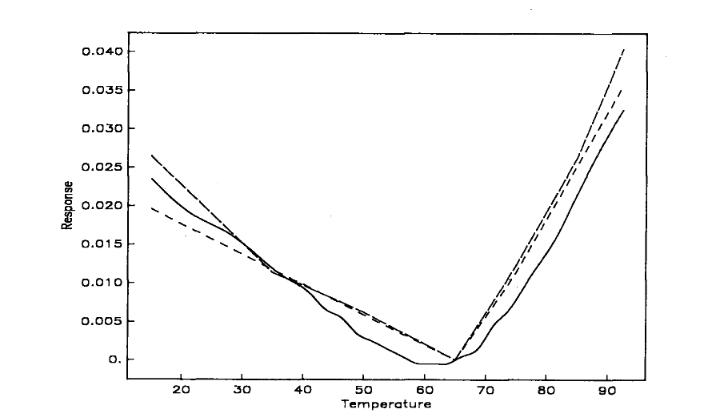
\includegraphics[scale=0.68]{graph1.png}

Figure 1: Engle et al. pg. 316
\\The data shows that there is a positive correlation between the temperature and use in electricity as well as total load. In our experiment we will be measuring exactly these variables but will only use natural occurring phenomena like wind, temperature, and cloud cover. Engle et al. article focused on the percent change, however, our model will focus on the actual correlation between these variables.


\section{Data-set Description and Analysis}\label{sec:3}
In this section we describe the results...

\subsection{Case 1}
An example of subsection...

\section{Methodology}\label{sec:4}
We worked hard, and achieved very little...

\newpage

\section{Experimental Results}\label{sec:5}

Write all the results here!

\section{Conclusion and Discussion}\label{sec:6}



\bibliographystyle{apalike} 
\bibliography{referencias.bib} 
https://www.tandfonline.com/doi/pdf/10.1080/01621459.1986.10478274?needAccess=true

\end{document}
